\documentclass[a4paper, french]{article}
\usepackage{config}
\author{Vincent Commin \& Louis Leenart}
\date{\today}
\setcounter{secnumdepth}{6}
\begin{document}

\begin{titlepage}
    \begin{flushleft}
        \includegraphics[width=5cm]{UL.jpg}\par
        \centering
        
        \vspace{13\baselineskip}       
        \HRule \\[0.4cm]

        {\Huge 
        GIF-4104 - TP 2\par}
        \vspace{0.4cm}
        \HRule
        \vfill
        Équipe 1 : Vincent Commin \& Louis Leenart\medskip \par
    \end{flushleft}
\end{titlepage}

\newpage
\section{Introduction}

Pour ce deuxième TP, nous avons du reprendre notre approche de parallélisation de recherche de
nombre premiers, en utilisant cette fois \textbf{OpenMP} au lieu de \textbf{pthread}. Nous utilisons
cependant encore une fois l'algorithme de
\href{https://fr.wikipedia.org/wiki/Test_de_primalit%C3%A9_de_Miller-Rabin}{\textit{\underline{Miller-Rabin}}}, et plus 
précisément l'implémentation de Stigen Larsen disponible sur
\href{https://github.com/cslarsen/miller-rabin}{\textit{\underline{Github}}}. Nous avons modifié
légerement cette implémentation afin de permettre la parallélisation ainsi qu'améliorer les
performances. Enfin, notre algorithme supporte la recherche sur les grands notre, via la librairie
\href{https://gmplib.org/}{\textit{\underline{GMP}}}. \\\\\\

\section{Notre approche}

Dans ce TP, nous avons fait de notre mieux pour paralléliser notre algorithme en simplifiant un
maximum la lecture du code, tout en donnant des performances satisfaisantes. L'utilisation
d'OpenMP a permi de rendre le code beaucoup plus concis. \\\\

L'algorithme que nous avons mis en place est le suivant : 

\begin{lstlisting}[style=txt] 
premiers : vecteur de grands nombres 
intervals : vecteur de pair de grands nombres
nb_threads : entier
tours : entier

// Section parallélisée sur nb_threads
POUR i ALLANT DE 0 A size(intervals) FAIRE
    local_premiers : vecteur de grand nombres
    pair : pair de grands nombres = intervals[i]
    aleatoire : generateur de nombre premier

    POUR j ALLANT DE pair.borne_basse A pair.borne_haute FAIRE
        est_premier : booléen = calculer_premier(j, tours, aleatoire)
        SI est_premier ALORS
            AJOUTER j DANS local_premiers
        FIN SI
    FIN POUR

    FUSIONNER local_premiers DANS premiers
FIN POUR
\end{lstlisting}

Aussi, afin de maximiser les performances, nous utilisons une fusion des intervals pour limiter la
duplication des calculs. En effet, si deux intervals se chevauchent, alors ils sont réunis en un
seul. Nous nous sommes inspirés de l'approche évoqué par l'équipe 3 dans leur rapport, et avons
implémenté notre propre algorithme adapté à notre structure de données.

\newpage

\section{Machine utilisée pour les tests de performance}

\begin{center}
    \begin{tabularx}{0.45\textwidth}{|>{\raggedleft\arraybackslash}X|>{\raggedright\arraybackslash}X|}
        \hline
        Modèle & intel i7-8550U \\
        \hline
        Architecture & x86\_64 \\
        \hline
        OS & Archlinux \\
        \hline
        Fréquence CPU & 3.4GHz \\
        \hline
        C\oe urs physiques & 4 \\
        \hline
        C\oe urs logiques & 8 \\
        \hline
        Ram & 16 Go, 2400 $MT/s$ \\
        \hline
    \end{tabularx}
\end{center}

\section{Résultats obtenus}

\begin{center}
    \begin{tabularx}{\textwidth}{l r}
        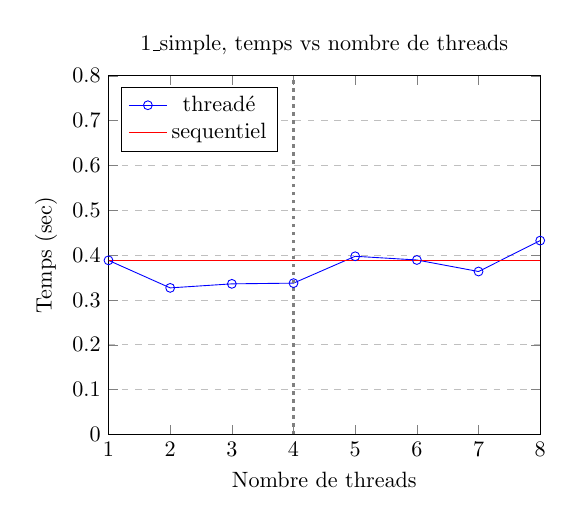
\begin{tikzpicture}[scale=0.8, transform shape]
            \begin{axis}[
                title={1\_simple, temps vs nombre de threads},
                xlabel={Nombre de threads},
                ylabel={Temps (sec)},
                xmin=1, xmax=8,
                ymin=0, ymax=0.8,
                xtick={1,2,3,4,5,6,7,8},
                ytick={0, 0.1, 0.2, 0.3, 0.4, 0.5, 0.6, 0.7, 0.8},
                legend pos=north west,
                ymajorgrids=true,
                grid style=dashed,
                ]        
                \addplot[color=blue, mark=o] coordinates {(1, 0.388412)(2, 0.327019)(3, 0.336002)(4, 0.337597)(5, 0.397522)(6, 0.389236)(7, 0.363555)(8, 0.432505)};   
                \addplot[color=red, mark=] coordinates {(1, 0.388412)(8, 0.388412)};
                \addplot[color=gray, dotted, ultra thick] coordinates {(4, 0)(4, 0.8)};
                \legend{threadé, sequentiel}
            \end{axis}
        \end{tikzpicture}
        &
        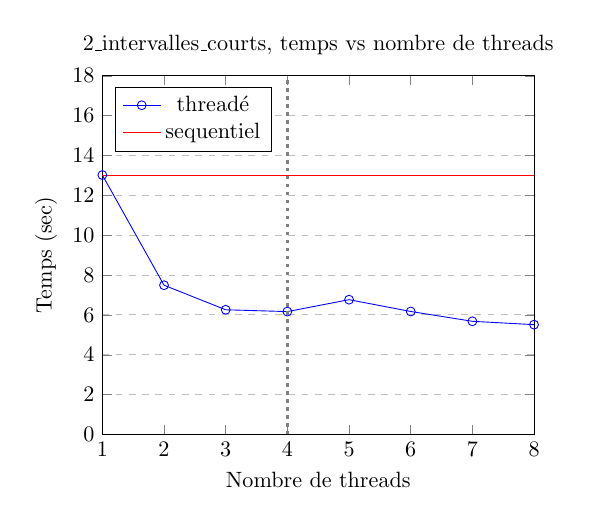
\begin{tikzpicture}[scale=0.8, transform shape]
            \begin{axis}[
                title={2\_intervalles\_courts, temps vs nombre de threads},
                xlabel={Nombre de threads},
                ylabel={Temps (sec)},
                xmin=1, xmax=8,
                ymin=0, ymax=18,
                xtick={1,2,3,4,5,6,7,8},
                ytick={0, 2, 4, 6, 8, 10, 12, 14, 16, 18},
                legend pos=north west,
                ymajorgrids=true,
                grid style=dashed,
                ]        
                \addplot[color=blue, mark=o] coordinates {(1, 13.0218)(2, 7.49222)(3, 6.25925)(4, 6.16795)(5, 6.76602)(6, 6.17349)(7, 5.68115)(8, 5.51193)};        
                \addplot[color=red, mark=] coordinates {(1, 13.0218)(8, 13.0218)};
                \addplot[color=gray, dotted, ultra thick] coordinates {(4, 0)(4, 18)};
                \legend{threadé, sequentiel}
            \end{axis}
        \end{tikzpicture}
        \\ 
        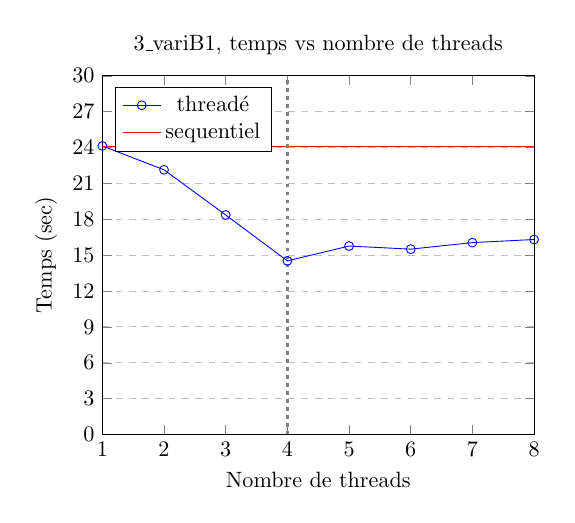
\begin{tikzpicture}[scale=0.8, transform shape]
            \begin{axis}[
                title={3\_variB1, temps vs nombre de threads},
                xlabel={Nombre de threads},
                ylabel={Temps (sec)},
                xmin=1, xmax=8,
                ymin=0, ymax=30,
                xtick={1,2,3,4,5,6,7,8},
                ytick={0, 3, 6, 9, 12, 15, 18, 21, 24, 27, 30},
                legend pos=north west,
                ymajorgrids=true,
                grid style=dashed,
                ]        
                \addplot[color=blue, mark=o] coordinates {(1, 24.1355)(2, 22.1384)(3, 18.3632)(4, 14.5218)(5, 15.7618)(6, 15.5036)(7, 16.0504)(8, 16.3093)};        
                \addplot[color=red, mark=] coordinates {(1, 24.1355)(8, 24.1355)};
                \addplot[color=gray, dotted, ultra thick] coordinates {(4, 0)(4, 30)};
                \legend{threadé, sequentiel}
            \end{axis}
        \end{tikzpicture}
        &
        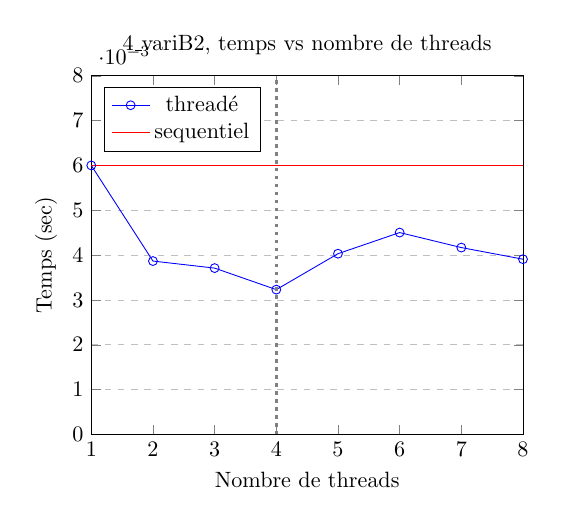
\begin{tikzpicture}[scale=0.8, transform shape]
            \begin{axis}[
                title={4\_variB2, temps vs nombre de threads},
                xlabel={Nombre de threads},
                ylabel={Temps (sec)},
                xmin=1, xmax=8,
                ymin=0, ymax=0.008,
                xtick={1,2,3,4,5,6,7,8},
                ytick={0, 0.001, 0.002, 0.003, 0.004, 0.005, 0.006, 0.007, 0.008},
                legend pos=north west,
                ymajorgrids=true,
                grid style=dashed,
                ]        
                \addplot[color=blue, mark=o] coordinates {(1, 0.00600104)(2, 0.00386856)(3, 0.00371145)(4, 0.00323145)(5, 0.0040326)(6, 0.00450418)(7, 0.00416944)(8, 0.00391003)};        
                \addplot[color=red, mark=] coordinates {(1, 0.00600104)(8, 0.00600104)};
                \addplot[color=gray, dotted, ultra thick] coordinates {(4, 0)(4, 0.008)};
                \legend{threadé, sequentiel}
            \end{axis}
        \end{tikzpicture}
    \end{tabularx}
\end{center}

\newpage

\begin{center}
    \begin{tabularx}{\textwidth}{l r}
        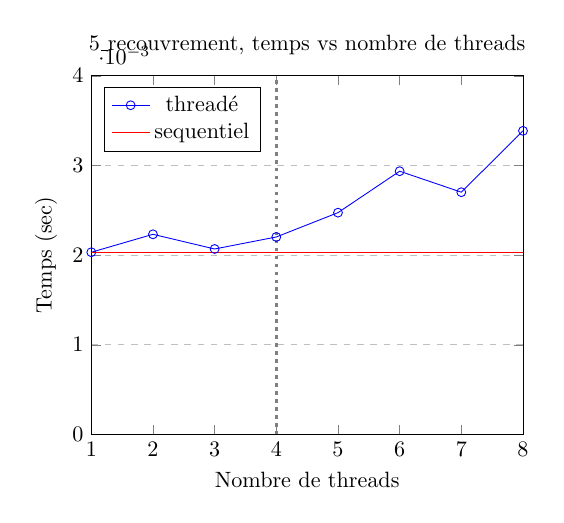
\begin{tikzpicture}[scale=0.8, transform shape]
            \begin{axis}[
                title={5\_recouvrement, temps vs nombre de threads},
                xlabel={Nombre de threads},
                ylabel={Temps (sec)},
                xmin=1, xmax=8,
                ymin=0, ymax=0.004,
                xtick={1,2,3,4,5,6,7,8},
                ytick={0, 0.001, 0.002, 0.003, 0.004},
                legend pos=north west,
                ymajorgrids=true,
                grid style=dashed,
                ]        
                \addplot[color=blue, mark=o]
                coordinates {(1, 0.00203256)(2, 0.00223267)(3, 0.00206891)(4, 0.00220282)(5, 0.00247404)(6, 0.00293645)(7, 0.00270223)(8, 0.00338652)};        
                \addplot[color=red, mark=] coordinates {(1, 0.00203256)(8, 0.00203256)};
                \addplot[color=gray, dotted, ultra thick] coordinates {(4, 0)(4, 0.004)};
                \legend{threadé, sequentiel}
            \end{axis}
        \end{tikzpicture}
        &
        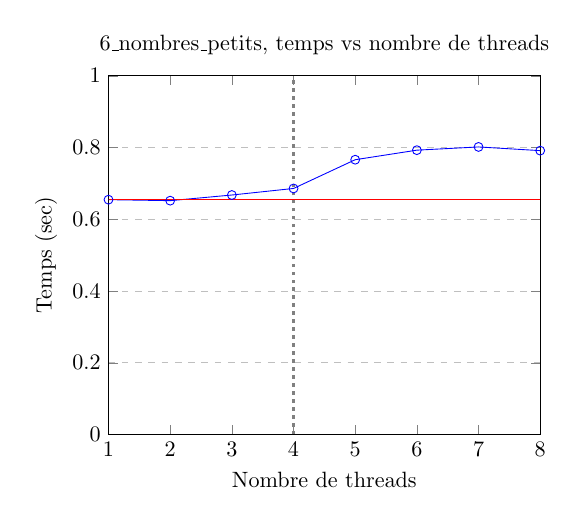
\begin{tikzpicture}[scale=0.8, transform shape]
            \begin{axis}[
                title={6\_nombres\_petits, temps vs nombre de threads},
                xlabel={Nombre de threads},
                ylabel={Temps (sec)},
                xmin=1, xmax=8,
                ymin=0, ymax=1,
                xtick={1,2,3,4,5,6,7,8},
                ytick={0, 0.2, 0.4, 0.6, 0.8, 1},
                legend pos=north west,
                ymajorgrids=true,
                grid style=dashed,
                ]        
                \addplot[color=blue, mark=o] coordinates {(1, 0.654738)(2, 0.651952)(3, 0.667715)(4, 0.685957)(5, 0.766144)(6, 0.792763)(7, 0.801771)(8, 0.791428)};        
                \addplot[color=red, mark=] coordinates {(1, 0.654738)(8, 0.654738)};
                \addplot[color=gray, dotted, ultra thick] coordinates {(4, 0)(4, 1)};
            \end{axis}
        \end{tikzpicture}
        \\ 
        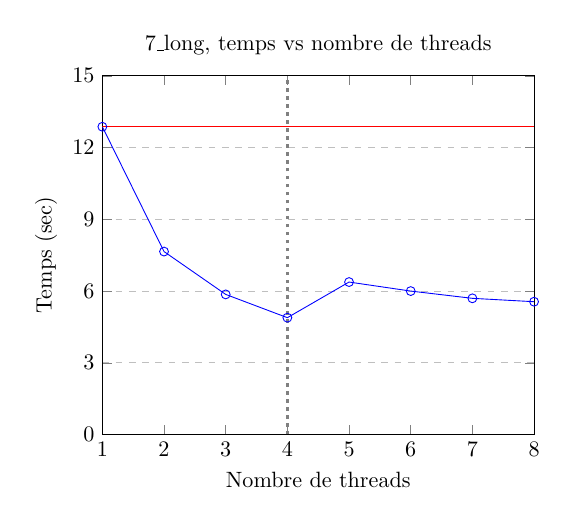
\begin{tikzpicture}[scale=0.8, transform shape]
            \begin{axis}[
                title={7\_long, temps vs nombre de threads},
                xlabel={Nombre de threads},
                ylabel={Temps (sec)},
                xmin=1, xmax=8,
                ymin=0, ymax=15,
                xtick={1,2,3,4,5,6,7,8},
                ytick={0, 3, 6, 9, 12, 15},
                legend pos=north west,
                ymajorgrids=true,
                grid style=dashed,
                ]        
                \addplot[color=blue, mark=o] coordinates {(1, 12.8705)(2, 7.65063)(3, 5.85883)(4, 4.88547)(5,6.37551)(6, 5.99824)(7, 5.69496)(8, 5.55317)};        
                \addplot[color=red, mark=] coordinates {(1, 12.8705)(8, 12.8705)};
                \addplot[color=gray, dotted, ultra thick] coordinates {(4, 0)(4, 15)};
            \end{axis}
        \end{tikzpicture}
        &
        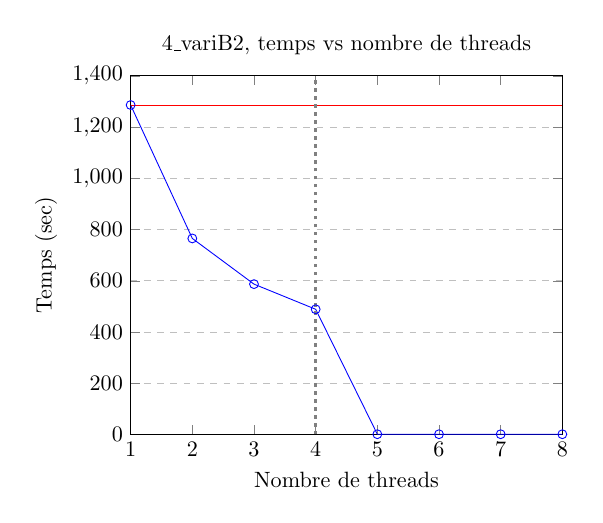
\begin{tikzpicture}[scale=0.8, transform shape]
            \begin{axis}[
                title={4\_variB2, temps vs nombre de threads},
                xlabel={Nombre de threads},
                ylabel={Temps (sec)},
                xmin=1, xmax=8,
                ymin=0, ymax=1400,
                xtick={1,2,3,4,5,6,7,8},
                ytick={0, 200, 400, 600, 800, 1000, 1200, 1400},
                legend pos=north west,
                ymajorgrids=true,
                grid style=dashed,
                ]        
                \addplot[color=blue, mark=o] coordinates {(1, 1286.07)(2, 765.321)(3, 586.961)(4, 488.817)(5, 1)(6, 1)(7, 1)(8, 1)};        
                \addplot[color=red, mark=] coordinates {(1, 1286.07)(8, 1286.07)};
                \addplot[color=gray, dotted, ultra thick] coordinates {(4, 0)(4, 1400)};
            \end{axis}
        \end{tikzpicture}
    \end{tabularx}
\end{center}

\section{Analyse}


\section{Conclusion}


\end{document}